Nach der gestrigen Durchfahrt, wollten wir uns heute das Todestal genauer ansehen.
Wir machten halt bei den Dünen, liefen die nähste und höchste hoch und mit fast verbrannten Füßen wieder runter.
Ein Hinweisschild wies einen darauf hin die Dünen nur am Morgen oder am Abend zu begehen.
Macht absolut Sinn.

\thispagestyle{empty}
\begin{tikzpicture}[remember picture, overlay]
\node[inner sep=0pt, yshift=.25\paperheight] at (current page.south) {%
	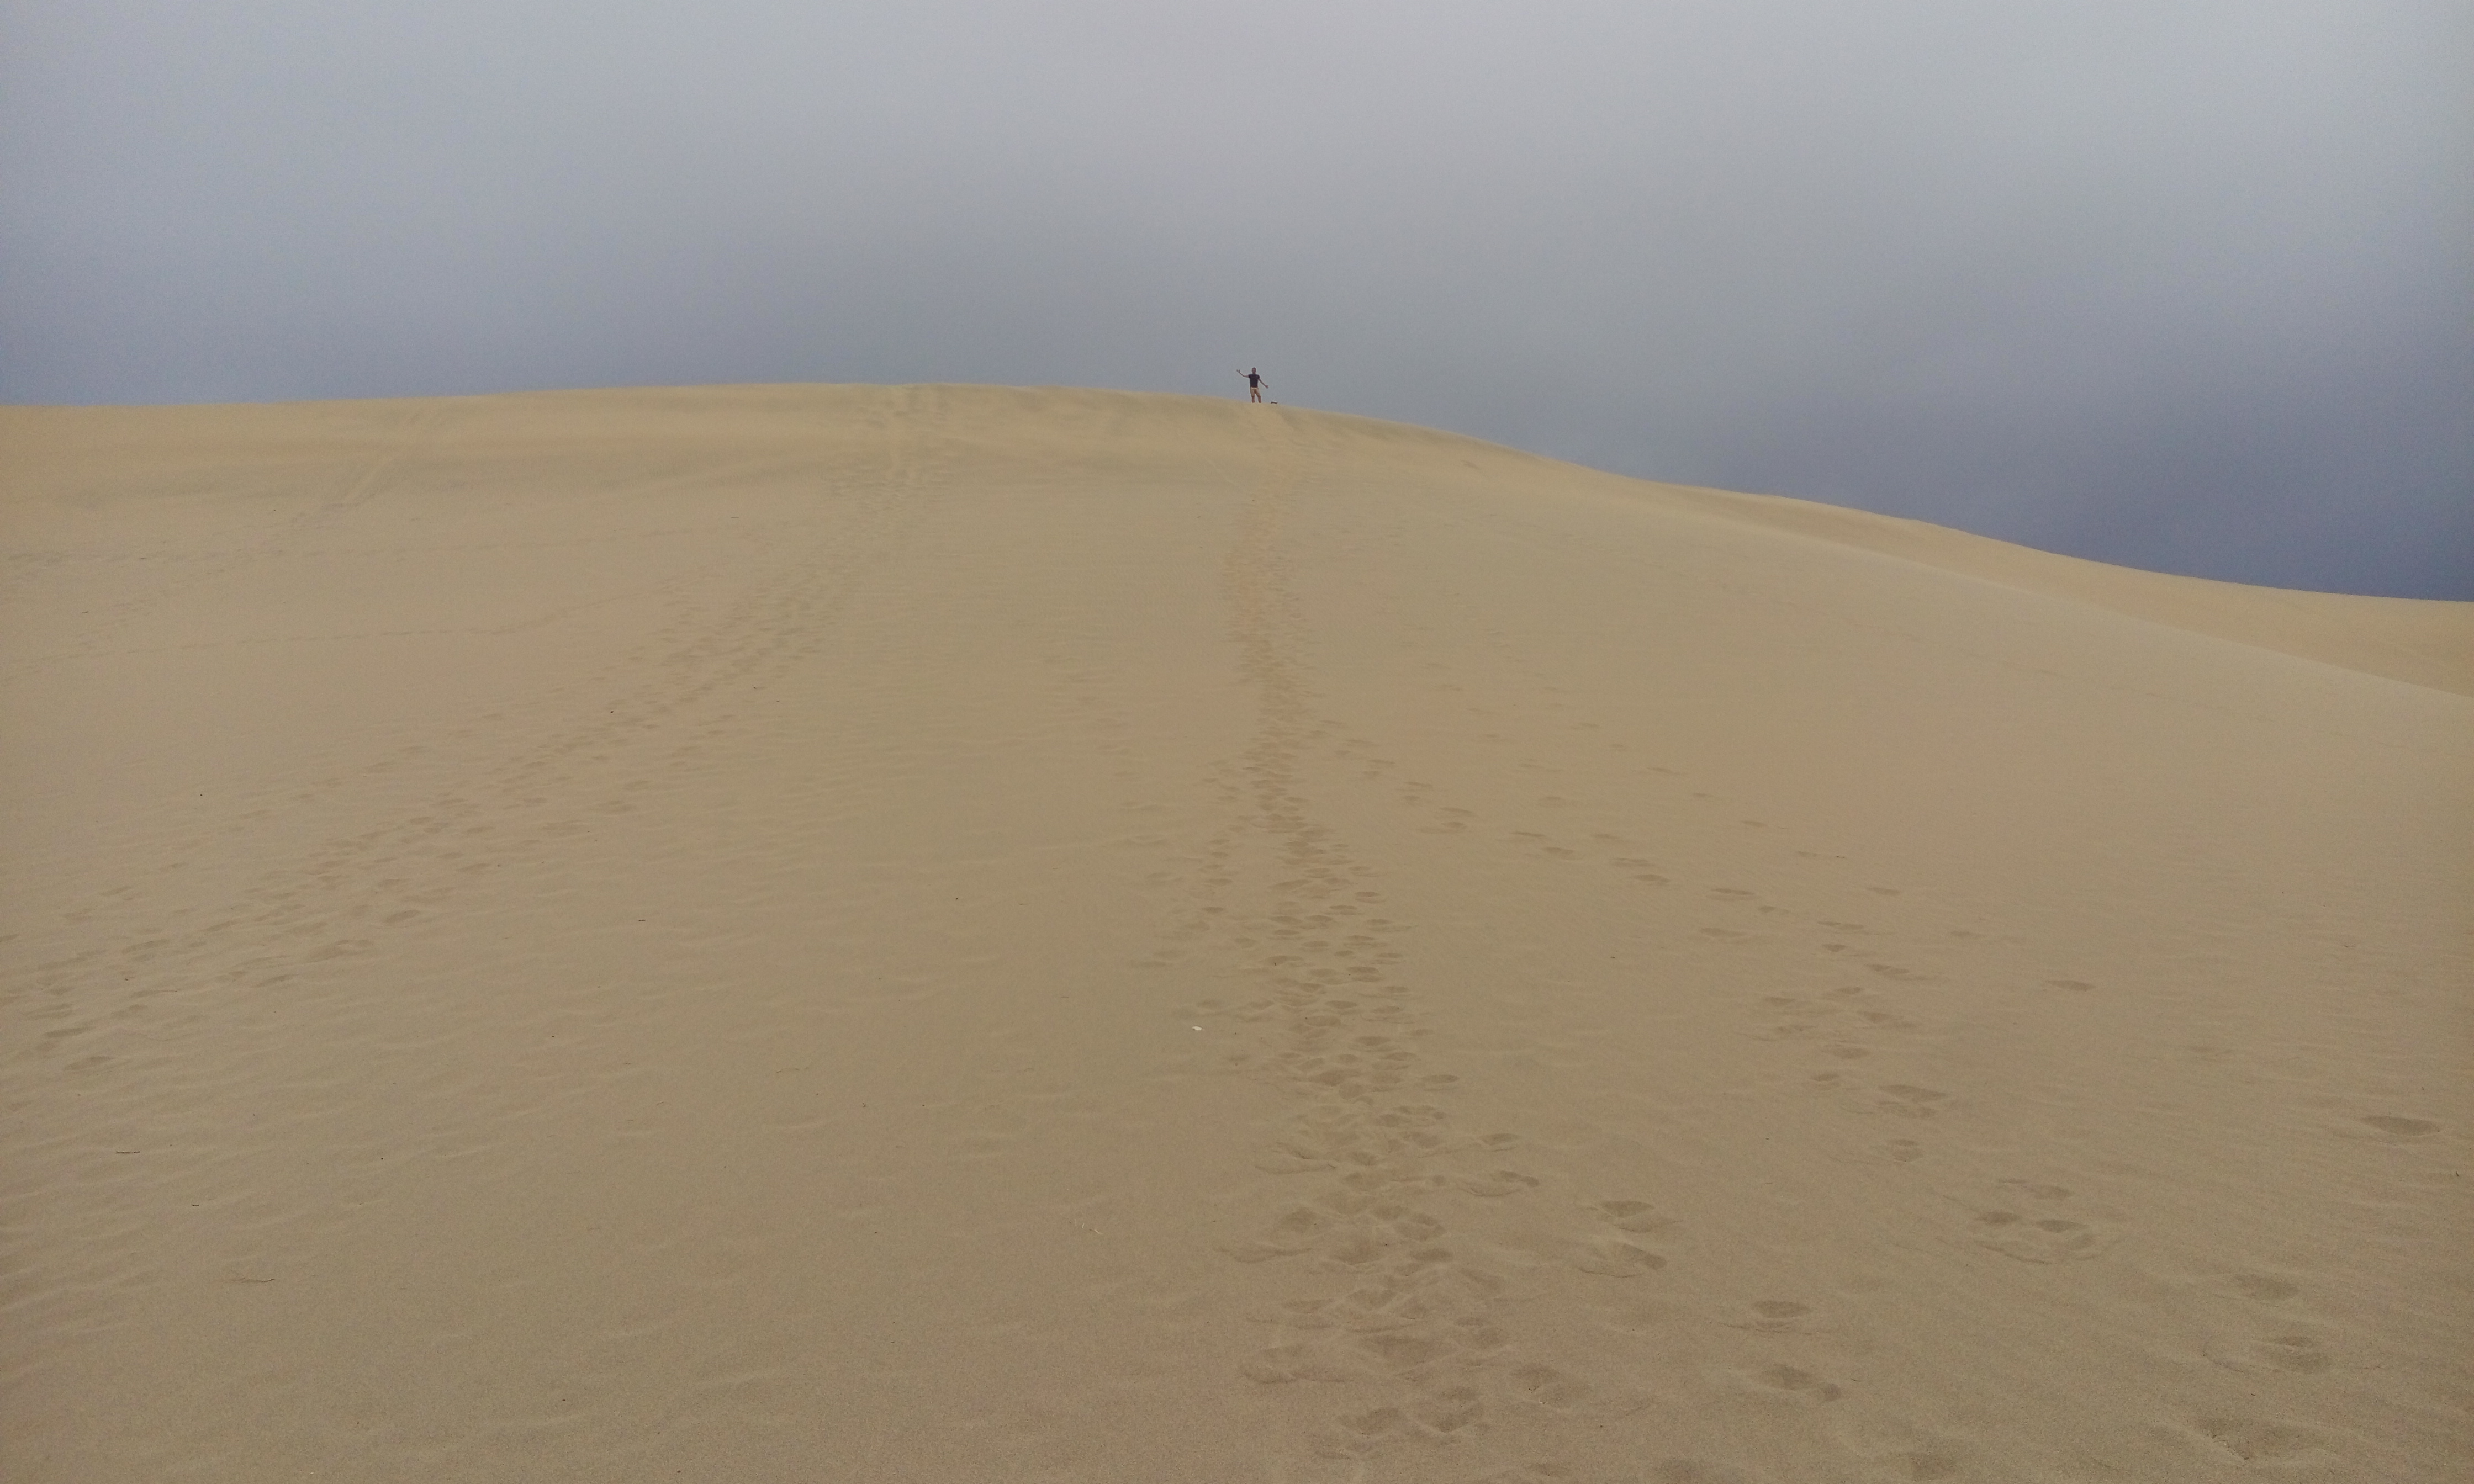
\includegraphics[angle=0,width=\paperwidth,height=.5\paperheight]{27/image20160427_111303992.jpg};%
};
\end{tikzpicture}
\newpage

Als nächstes hielten wir bei einer ehemaligen Abbaustätte, die sich nicht lange lohnte.
%Du hast doch sicherlich ein Foto und damit den Namen und worums da ging, oder?
Dann gab es noch ein obligatorisches Besucherzentrum und von dort fuhren wir erst einen Salzsee und anschließend \FOREIGN{Dante's View} an.
Bei \FOREIGN{Dante's View} blickt man auf den Salzsee, nur eben von einer erhöhten Position.

Als Nachtlager stand wieder Las Vegas an und so machten wir uns auf den Weg.
Statt auf die Schatzinsel verschlug es uns zum Zirkus.
Im Circus Circus war zum einen die Nacht spott billig, zum anderen hat das Hotel einen eigenen Freizeitpark mit Achterbahnen!

\thispagestyle{empty}
\begin{tikzpicture}[remember picture, overlay]
\node[inner sep=0pt, yshift=.25\paperheight] at (current page.south) {%
	\includegraphics[angle=0,width=\paperwidth,height=.5\paperheight]{27/image20160427_131909168.jpg};%
};
\end{tikzpicture}
\newpage

\thispagestyle{empty}
\begin{tikzpicture}[remember picture, overlay]
\node[inner sep=0pt, yshift=-.25\paperheight] at (current page.north) {%
	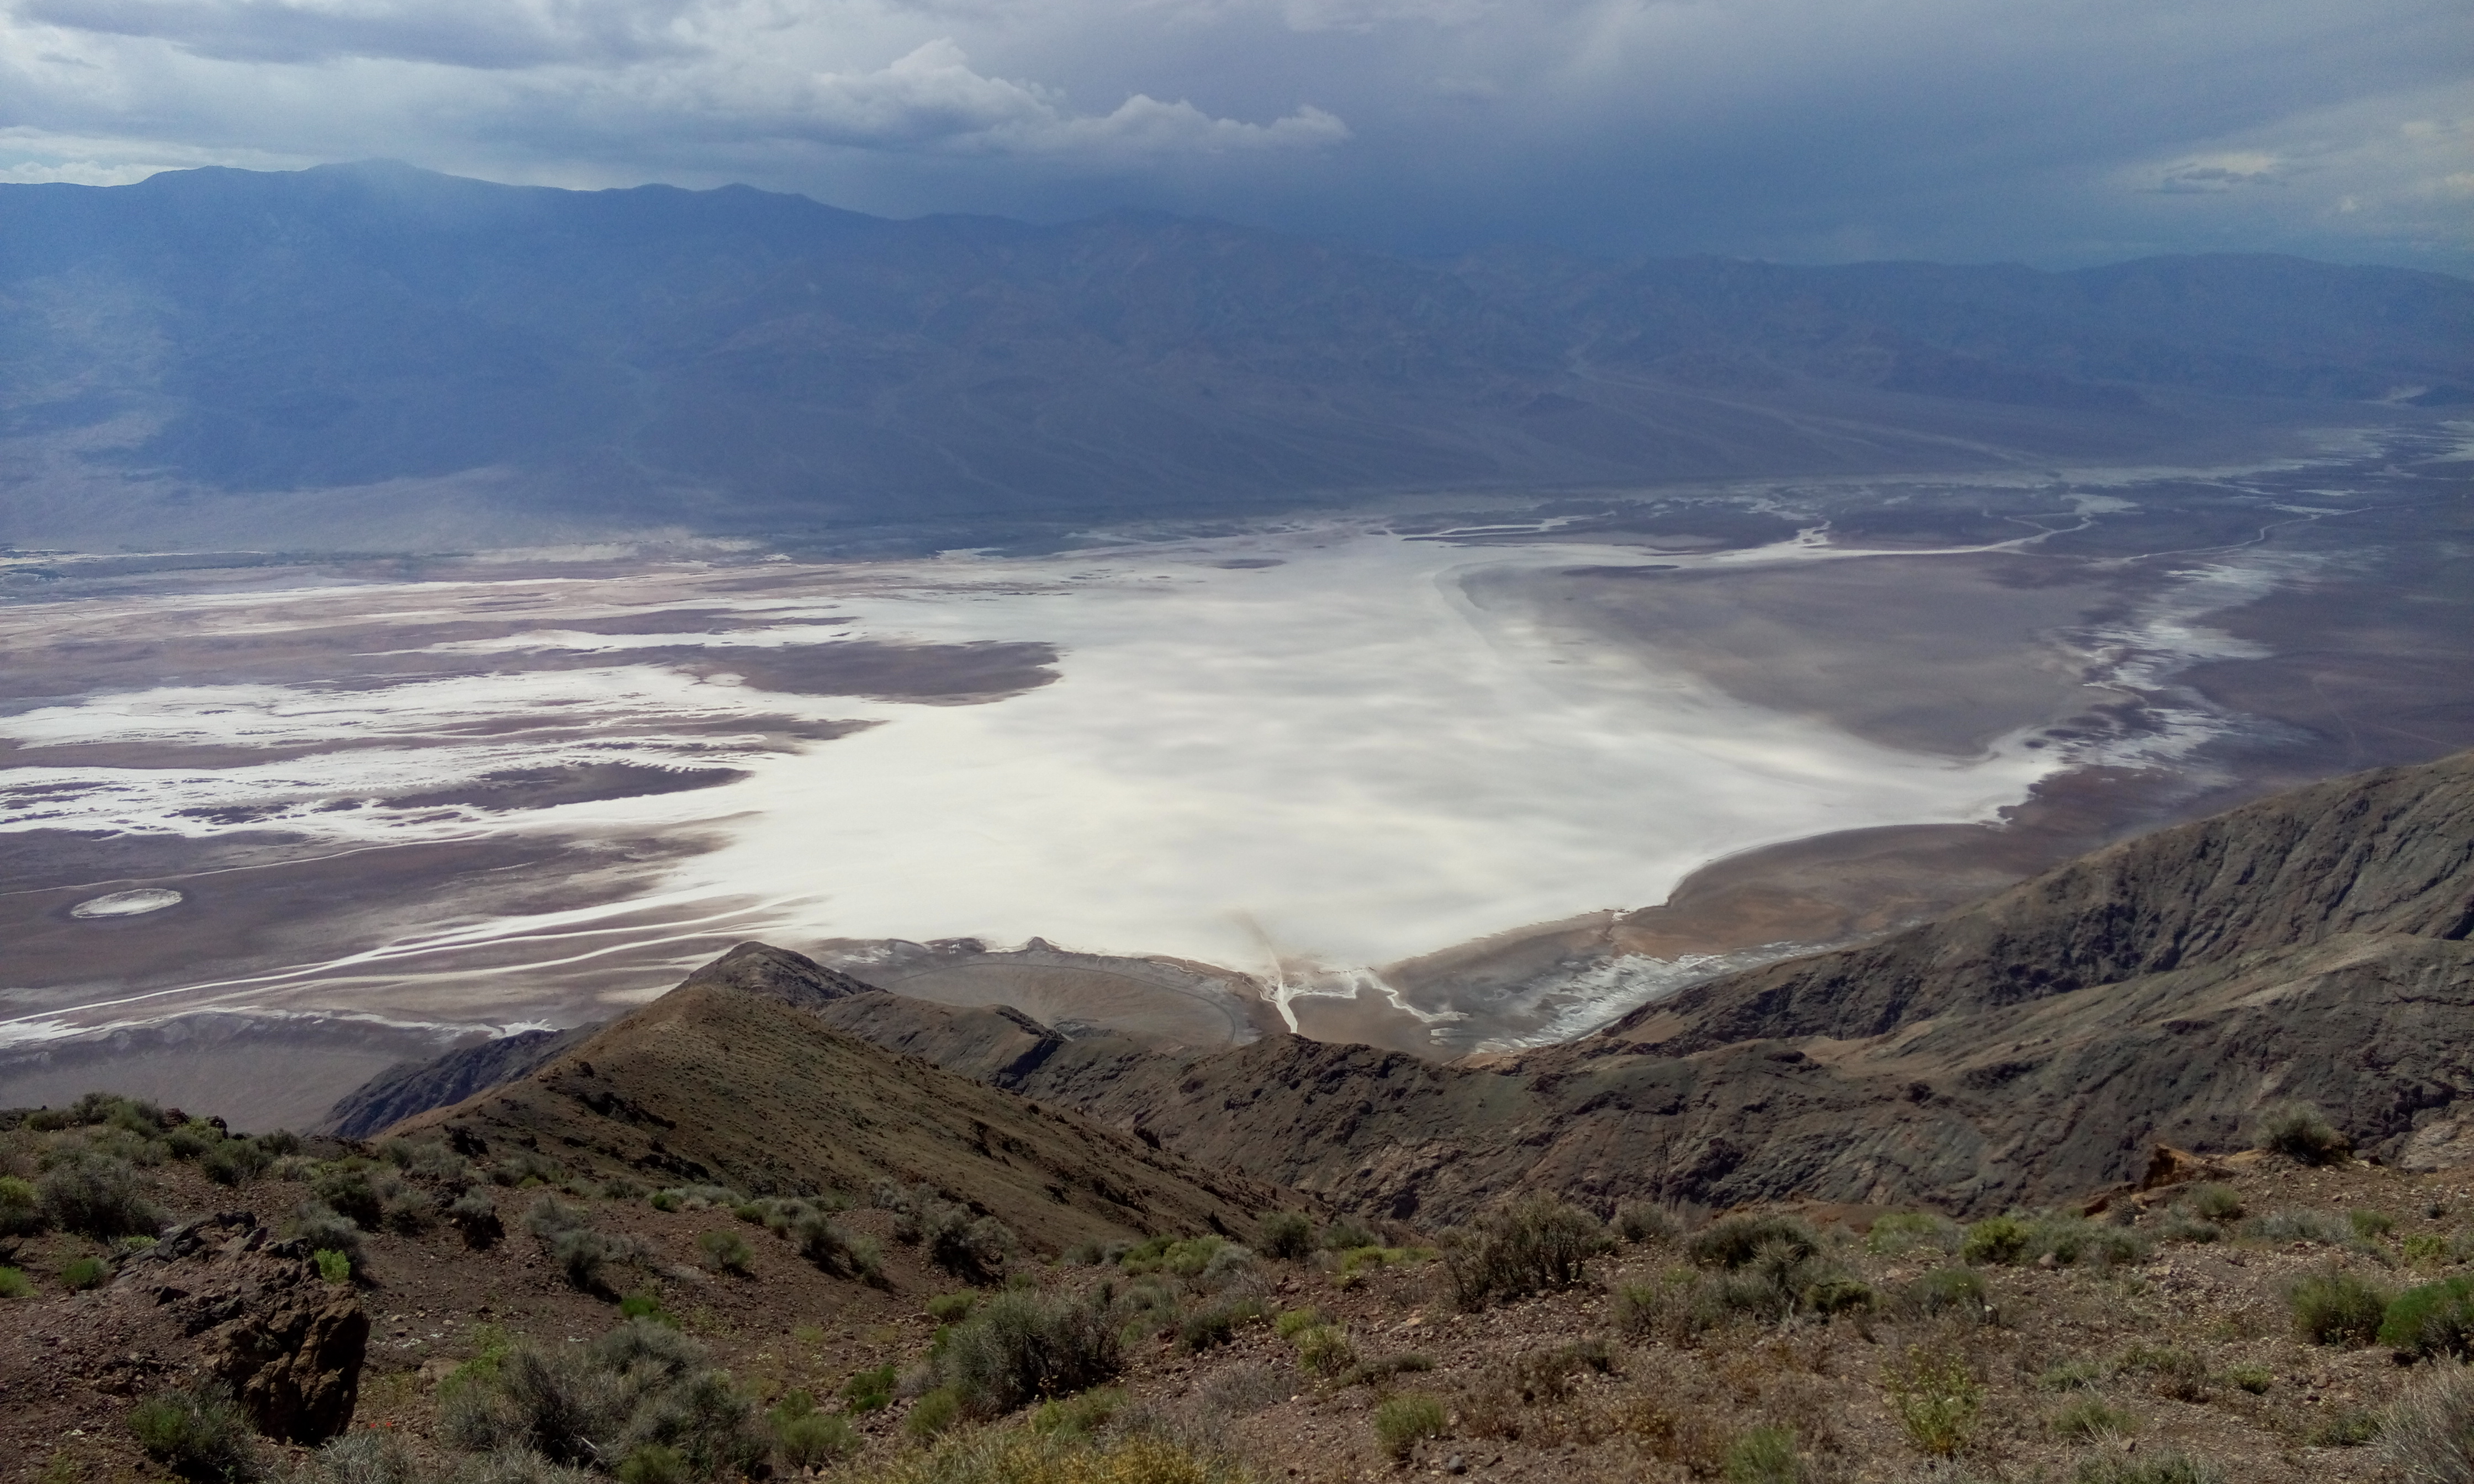
\includegraphics[angle=0,width=\paperwidth,height=.5\paperheight]{27/image20160427_144208822.jpg};%
};
\end{tikzpicture}

\vspace*{.4\paperheight}

Am Abend sind wir nochmal um die Häuser gezogen und haben mal wieder Ausländer angetroffen.
Dieses Mal Österreicher.
Die hatten am Vortag erfolgreich 10~\$ am Roulettetisch auf eine Zahl gesetzt und bestellten nun unbeschwerter.
